\section{Motivated Example}

\begin{figure}[htbp]
	\centering
	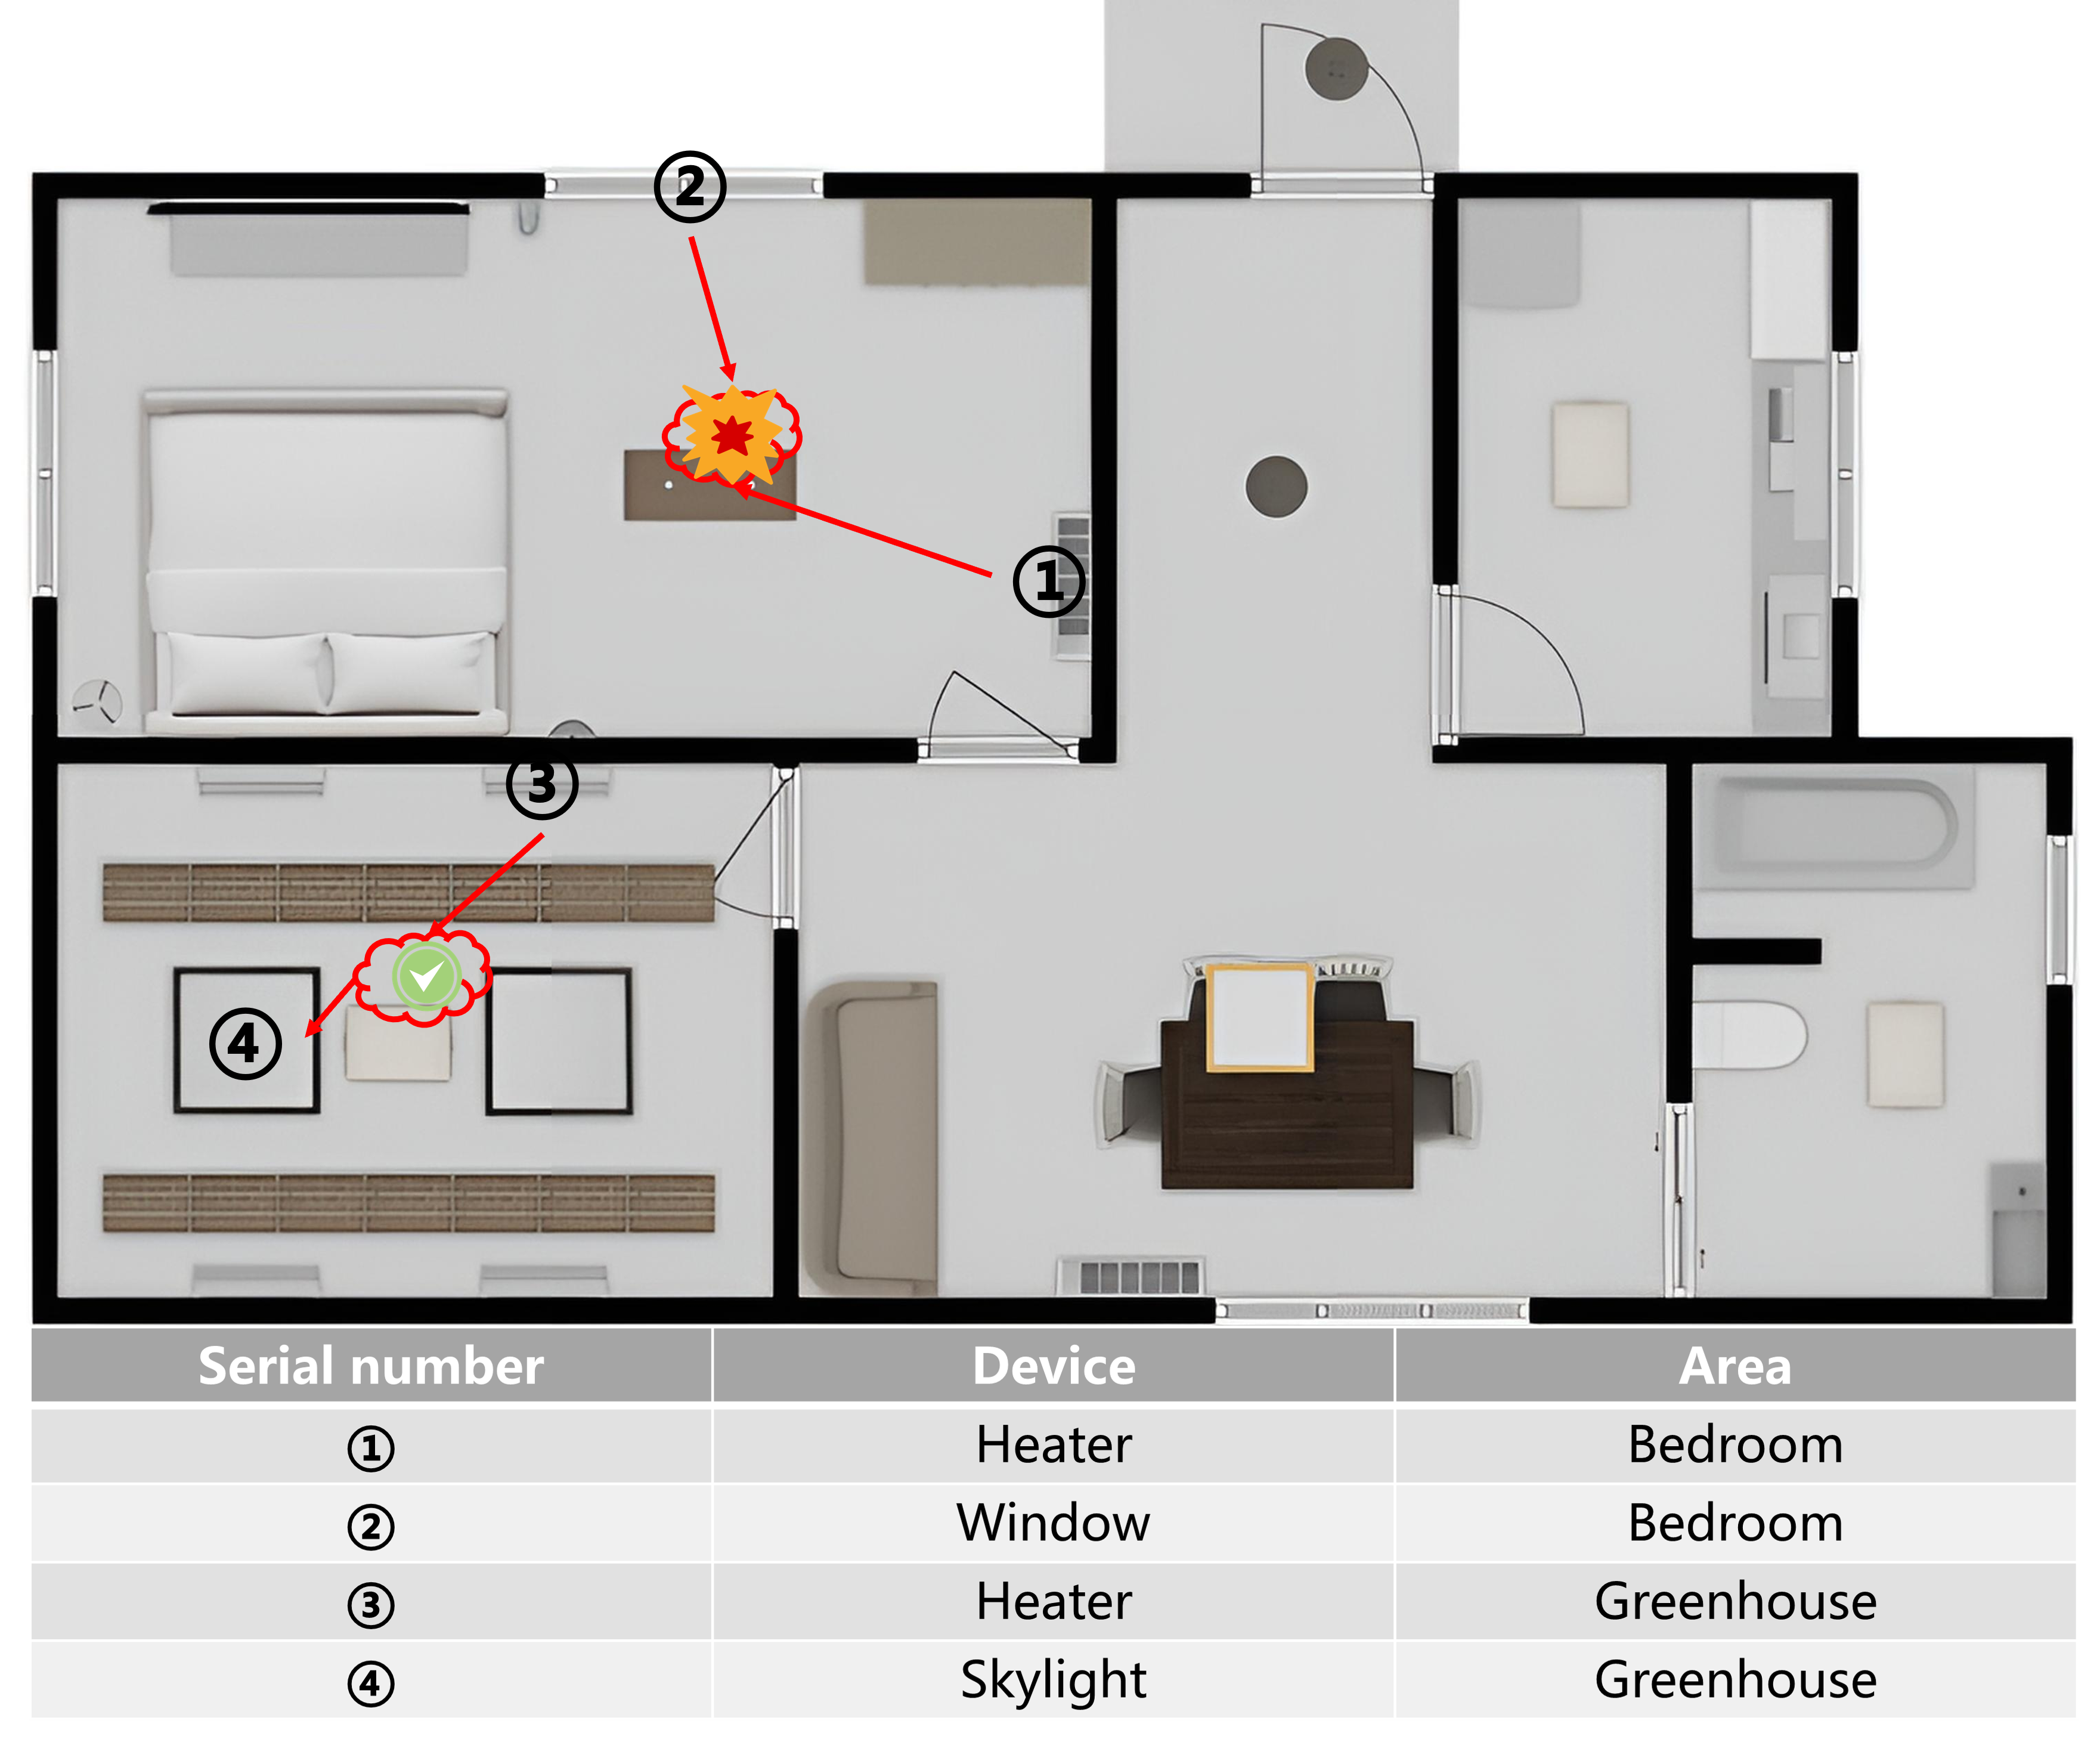
\includegraphics[width=0.4\textwidth]{figure/motivated_example.png}
	\caption{Motivated Example}
	\label{motivated_example}
\end{figure}

%这一章节将使用具体实例来展示规则冲突的一些性质以及当前规则冲突检测与环节方法存在的缺陷。Fig.\ref{smarthome_floorplan}展示了一个智能家居平面图,共包括Outdoor(中间上方)、porch(中间)、living room(中间下侧)、 kitchen(中间右侧)、batch room(右下侧)、 bedroom(中间左侧)和green house(garden,左下侧)7个区域。
In this section, specific examples will be used to demonstrate some properties of rule conflicts, as well as the shortcomings of current rule conflict detection and mitigation methods. Fig. \ref{motivated_example} shows a smart home floor plan, including seven areas: Outdoor (top center), porch (center), living room (bottom center), kitchen (bottom right), batch room (bottom right), bedroom (center left), and green house (garden, bottom left).

%在green house中设定自动化规则1,触发条件为\texttt{日落},执行动作是\texttt{打开加热器}。同时设定自动化规则2,触发条件为\texttt{温度达到三十摄氏度},执行动作是\texttt{打开窗户并关闭加热器}。如Fig.\ref{motivated_example}中左下角展示的那样,当日落时在green house中首先自动执行了规则1,加热器打开为green house持续供暖,温度持续上升可能超过30摄氏度,此时自动化规则1的执行结果通过影响室内温度从而触发自动化规则2的执行,使得加热器关闭并且打开天窗。在green house中打开天窗往往是符合用户预期且安全的,但是如果这两条规则设置在用户的卧室中,则情况会明显不同:规则1通过提高卧室温度触发规则2的执行,打开,了卧室的窗户,卧室的窗户往往不是天窗,而且如果在用户预期之外打开卧室窗户则会给智能家居系统引入安全隐患,甚至被攻击者恶意利用规则从而创造规则执行的通路来控制窗户、门锁等安全敏感设备。
In the greenhouse, automation rule 1 is set with the trigger condition being \texttt{sunset}, and the action is \texttt{turn on the heater}. Simultaneously, automation rule 2 is set with the trigger condition being \texttt{temperature reaches thirty degrees Celsius}, and the action is \texttt{open the windows and turn off the heater}. As shown in the bottom left corner of Fig.\ref{motivated_example}, when the sun sets in the greenhouse, rule 1 is automatically executed first, and the heater is turned on to continuously provide heat to the greenhouse. The temperature may continue to rise above 30 degrees Celsius. At this time, the execution result of automation rule 1 affects the indoor temperature, thereby triggering the execution of automation rule 2, which turns off the heater and opens the skylight. Opening the skylight in the greenhouse is often in line with user expectations and is safe. However, if these two rules are set in the user's bedroom, the situation will be significantly different: rule 1 triggers the execution of rule 2 by raising the bedroom temperature, opening the windows of the bedroom. The windows of the bedroom are often not skylights, and opening the bedroom windows unexpectedly can introduce security risks to the smart home system, and attackers may even maliciously use the rules to create execution paths to control security-sensitive devices such as windows and door locks.

%以上示例表明,规则交互可能并非由一条规则的执行动作直接影响另一条规则(例如两条同时执行的规则,一个控制空调为加热模式,一个控制空调为制冷模式),也可能通过间接通道产生交互(常见的有温度、湿度、亮度、声音等等),在检测规则冲突时需要考虑到源于其它通道的规则冲突。同时还能观察到规则冲突具有区域性和用户的主观性。以上规则交互如果发生在green house就不被视为规则冲突,发生在卧室则可能被视为规则冲突,用户的主观性体现在针对一对规则交互,有的用户可能将其视为规则冲突,有的用户认为是正常的规则交互(例如卧室空调的除湿模式和加湿器交替工作维持空气湿度保持在适宜的水平,有的用户认为是正常交互,还有用户可能会认为是浪费资源)。除此之外,上述示例还能表明在智能家居系统中对侧面通道的检测不能仅仅通过温度、湿度等参数界定,还应该具有区域属性,例如porch的灯光可能影响到厨房和客厅的亮度、却并不会影响到卧室的亮度,如果两个与亮度相关的规则同时执行可能并不会发生交互。
The above examples show that rule interactions may not be directly influenced by the execution action of one rule on another (e.g., two rules executing simultaneously, one controlling the air conditioner to heat mode and the other to cool mode), but may also be generated through indirect channels (commonly temperature, humidity, brightness, sound, etc.). When detecting rule conflicts, it is necessary to consider rule conflicts originating from other channels. At the same time, it can be observed that rule conflicts have regionality and user subjectivity. The above rule interaction may not be regarded as a rule conflict if it occurs in a greenhouse, but it may be regarded as a rule conflict if it occurs in a bedroom. User subjectivity is reflected in the fact that for a pair of rule interactions, some users may regard it as a rule conflict, while others may regard it as a normal rule interaction (for example, the dehumidification mode of the bedroom air conditioner and the humidifier work alternately to maintain the air humidity at a suitable level, some users think it is a normal interaction, while others may think it is a waste of resources). In addition, the above examples also show that the detection of side channels in smart home systems should not be limited to temperature, humidity and other parameters, but should also have regional attributes. For example, the porch lights may affect the brightness of the kitchen and living room, but will not affect the brightness of the bedroom. If two brightness-related rules are executed at the same time, they may not interact with each other.

%针对以上示例,如果采用特定的安全策略的方法进行检测需要用户付出大量的effort,因为不同家庭因为户型、设备等差异性导致不同的家庭都需要相关专业人员设定所有安全策略,且安全策略很可能包含所有的规则冲突。如果根据自动化规则交互模式进行判断,确实能够检测到卧室中发生的规则冲突,但是也会将green house中的规则交互视为规则冲突,当设定的自动化规则数量增多,容易产生大量的误报需要用户逐个确认,也会导致较大的user's effort。
It requires a lot of effort for users to set all security policies using specific security strategies to detect potential risks, because different families need relevant professionals to set all security policies due to differences in housing types, equipment, etc., and security policies are likely to contain all rule conflicts. If the judgment is made based on the automatic rule interaction mode, the rule conflict that occurs in the bedroom can indeed be detected, but the rule interaction in the green house will also be regarded as a rule conflict. When the number of set automatic rules increases, a large number of false positives are likely to occur and need to be confirmed by users one by one, which will also lead to a large user's effort.